\chapter {Formation of Planetary Embryos in the Inner Solar System}

\section{Introduction} \label{sec:intro}

The standard scenario of terrestrial planet formation involves the pairwise accretion of small rocky bodies, called planetesimals, 
that condense from dust out of the protostellar disc \cite{safronov69}. This accretion process can be broken into a series of 
distinct stages. First, dust particles settle toward the midplane of the disc and clump together via gravitational instability 
\cite{goldreich73, youdin02}, streaming instabilities \cite{johansen07, johansen15}, turbulent concentration 
\cite{chambers10, cuzzi08, cuzzi10, hopkins16} or direct sticking \cite{okuzumi12, windmark12, garaud13, katoka13}. These 
formation models predict a wide variation in the initial size of planetesimals, ranging from hundreds of meters up to a few 
hundred kilometers in diameter.

After this condensation process ends, growth continues via pairwise collisions between planetesimals. Above about 1 km in size, 
gravitational focusing becomes effective and the collision rate strongly increases. This marks the beginning of the intermediate 
stage of accretion. During this phase, runaway growth \cite{duncan89, kokubo96, barnes09} quickly increases the size of the 
largest bodies. Eventually, the largest bodies grow massive enough to heat the small planetesimals, which then inhibits the 
runaway growth effect. This marks the transition into the phase of oligarchic growth in which the handful of large bodies all tend 
to grow at the same rate. This produces a bimodal size distribution of planetesimals, with many small bodies and a handful of 
very large bodies. During this phase, a combination of scattering events between the oligarchs and dynamical friction from the 
small planetesimals places the oligarchs on nearly circular orbits that are spaced apart by approximately 5-10 Hill radii 
\cite{kokubo98}. Eventually, the oligarchs accrete most of the available material in the vicinity of their orbit, which eventually 
throttles their growth rate. On much longer time scales, the large bodies perturb each other onto crossing orbits, forming Mars to 
Earth sized bodies via occasional collisions. This phase of late stage accretion is highly chaotic and takes much longer to play 
out than the previous stages \cite{chambers98, raymond06}.

Generally, planetesimal accretion models fail to produce a configuration of planets that resembles that of the Solar System. 
Planets produced in the vicinity of Mars are systematically too massive \cite{wetherill92, raymond09, morishima10, izidoro15} 
and the terrestrial planets that form are too eccentric compared to their Solar System counterparts 
\cite{chambers98, agnor99, chambers01}. In addition, the present day water content of Earth, along with the large D/H ratio of 
Venus \cite{donahue82} does not match with models of solids that condensed out of the Solar nebula at 1 AU.

These issues all have proposed solutions, which generally involve altering the initial conditions for late-stage
accretion simulations. The condition of the Solar System at the beginning of the late stage accretion phase is poorly constrained. 
This is mostly due to the fact that planetesimal formation, and therefore the intermediate accretion phase which produces the 
planetary embryos, is not well understood. Although the present day population of small Solar System bodies has continued to 
evolve since the end of the intermediate accretion phase, the current size frequency distribution (SFD) of asteroid belt and 
Kuiper belt objects contains some clues about the accretion history. \cite{morbidelli09} argued that the SFD of asteroid belt 
objects larger than 100 km in diameter has been largely unchanged, aside from a size independent depletion factor. 
\cite{duncan89} did a long term stability analysis of small Solar System objects and found that small bodies left over from 
accretion should still be largely unperturbed. For these reasons, it should be possible to connect observables in the Solar System to planetesimal formation theories by modeling only the intermediate stages of accretion.

There are two common ways to model planetesimal growth. A powerful approach is to use statistical methods to track the 
evolution of large groups of planetesimals. This is known as the particle-in-a-box method \cite{greenberg78, wetherill89}. The 
evolution of growth is followed by tracking planetesimals in discrete bins of mass and semi-major axis. This removes the need to 
calculate the motion of every individual body and allows very large collections of planetesimals to be followed. Unfortunately, the 
dynamics that governs the evolution of these bodies does not always naturally emerge with this approach. As an example, 
\cite{weidenschilling11} found that a careful treatment of three body encounters led to a different prediction for the initial size 
distribution of planetesimals near the asteroid belt. Additionally, the particle-in-a-box method is not well suited for studying 
oligarchic growth because the largest mass bins, which dominate the evolution in this stage, contain small numbers of bodies. 
Non-gravitational effects such as gas drag and fragmentation require extra care to implement self-consistently 
\cite{leinhardt08}, although it has been successfully done \cite{wetherill93, chambers01}. To alleviate some of these issues 
while still being able to model large populations, a newer hybrid approach, in which large bodies are treated as single entities 
and planetesimals are treated as statistical ensembles has been developed 
\cite{weidenschilling97, kenyon06, levison12, morishima15}.

The most reliable and straightforward approach is to use N-body methods to follow the evolution and growth of the planetesimals 
\cite{lecar86}. By tracking the individual motions of bodies, the dynamics governing their evolution naturally emerges, no matter 
what the distribution of bodies looks like. However, N-body simulations involving collision detection are extremely 
computationally expensive, which severely limits both the resolution and number of timesteps that can be achieved. This is why 
there are very few studies of runaway and oligarchic with direct N-body simulations in the literature 
\cite{kokubo96, kokubo98, kokubo02, barnes09}. Instead, N-body methods are most commonly used to study late stage 
accretion, where the self-gravity and collisional evolution of the residual planetesimals is largely unimportant 
\cite{chambers98, agnor99,  chambers01, obrien06, morbidelli09}.

To date, we are not aware of any N-body simulations that resolve both the runaway and oligarchic growth phase  with more than 
about $10^4$ particles. At this resolution, stochasticity likely has a significant influence on dynamical friction and resonances 
may not be sufficiently resolved. \cite{raymond06} found that insufficient planetesimal resolution during the oligarchic growth 
phase limits the effectiveness of dynamical friction felt by the oligarchs, producing a population of embryos with unrealistically 
high eccentricities. This idea has also been applied to planet migration through a disc of planetesimals. \cite{cionco02} showed 
that resonances make a significant contribution to the dynamical friction torque exerted by the disc on the planet. This 
phenomenon requires the planetesimals to be finely resolved \cite{brunini07}. Dynamical friction is also facilitated via 
resonances in galactic dynamics \cite{lyndenbell72}. \cite{weinberg07a, weinberg07b} examined the effect of N-body particle 
counts on galaxy dynamics and showed that resonant interactions between the bar and halo were only effective with sufficient 
particle phase space coverage.

For these reasons, we motivate the need for a high resolution N-body simulation of planetesimal growth. We do this to better 
understand the effect that dynamical friction has on the intermediate stages of terrestrial planet growth and to examine what 
predictions a high resolution model makes about the residual population of planetesimals in the Solar System. In particular, 
resonances which are only effective with fine enough resolution, may have an important influence on planetesimal growth. In this 
paper, we investigate planetesimal evolution during the runaway and oligarchic growth phases with a direct N-body model. We 
begin by simulating an annulus of planetesimals with similar resolution to \cite{kokubo98} to validate our model. We then run the 
same configuration with 100x more particles to better understand the effects of resolution on the intermediate stages of 
terrestrial planet growth.

In section \ref{sec:sim}, we describe the simulation code that we use and provide a detailed description of the collision model. 
We also summarize the initial conditions used. In section \ref{sec:results}, we present the results of the low and high resolution 
simulation of terrestrial planet growth and highlight differences between the two. We find that a bump develops in the mass 
distribution of the high resolution simulation, which does not appear in the low resolution run. This feature manifests itself shortly 
after oligarchic growth commences and we infer that it is produced by extra heating via mean motion resonances between the 
oligarchs and small planetesimals. To further demonstrate this effect, we re-run the high resolution simulation with a narrower 
annulus (depopulating many of the resonances) and show that this reduces the prominence of the bump in the mass distribution. 
In section \ref{sec:dynfric}, we present a set of collisionless simulations of a planetary embryo embedded in an annulus of 
planetesimals. This more clearly demonstrates the differences in dynamical behavior between the low and high resolution 
models. In section \ref{sec:intermed}, we present two more simulations of planetesimal growth at intermediate resolutions and 
demonstrate that the location of the bump is sensitive to the initial planetesimal mass. Finally, section \ref{sec:discussion} 
connects these new results to our present understanding of terrestrial planet growth and we discuss the additional steps 
necessary to use our results to constrain the initial size of planetesimals in the Solar System.

\section{Simulations} \label{sec:sim}

\subsection{Numerical Methods} \label{sec:numerical}

All of the simulations described in this paper were performed with the highly parallel N-body code {\sc ChaNGa} . 
{\sc ChaNGa} is written in the {\sc CHARM++} programming language and has been shown to perform well when using up to 
half a million processors \cite{menon15} simultaneously. Gravitational forces are calculated using a modified Barnes-Hut tree 
algorithm with hexadecapole order expansions of the moments. For all of the simulations described in this paper, a node 
opening criterion of $\Theta_{BH}$ = 0.7 was used. \cite{richardson00} was able to resolve mean motion resonances in a 
terrestrial disc using a similar tree code with the same node opening criterion, so we expect that our model should properly 
handle resonance effects as well. The equations of motion are integrated using a kick-drift-kick leapfrog scheme. For more 
information about the implementation of {\sc ChaNGa} see \cite{jetley08}.

\subsection{Collision Model} \label{sec:collModel}

{\sc ChaNGa} is a smoothed particle hydrodynamics code originally designed for cosmology simulations. In order to use 
{\sc ChaNGa} to study planetesimal coagulation, we implemented a hard-body collision model that treats particles as solid 
objects with a fixed radius, rather than as smooth tracers of a fluid with a characteristic softening length. This work was largely 
based off of the hard body collision implementation in {\sc pkdgrav}, which is described in \cite{richardson94} and 
\cite{richardson00}.

Collisions are predicted at the beginning of each drift step by extrapolating the positions of the particles forward using the 
velocities calculated during the first kick. For each particle, the closest 64 neighbors are considered in the collision search. 
Because {\sc ChaNGa} is a tree code, the nearest neighbors of a particle can be retrieved in $\mathcal{O}(N\log{}N)$ time. After 
extrapolating the positions forward and checking for overlap with any neighbors, the earliest collision time $t_{coll}$ is stored for 
each particle.

After the prediction phase, particles with $t_{coll}$ less than the time step size $\Delta T$ must have their collisions resolved. For 
simplicity, all collisions in our simulations result in perfect accretion. \cite{ida93} showed that excluding the effects of 
fragmentation and collisional rebound does not qualitatively change the growth modes of the planetesimals. A merger between 
two particles of mass $m_{1}$ and $m_{2}$ results in a single particle of mass $M = m_{1} + m_{2}$, with the radius set to 
conserve density. The position and velocity of the resulting particle is set to the centre of mass position and velocity of the 
colliders at the moment of contact. The resulting merged particle is then drifted to the end of the step. If multiple collisions are 
predicted during a time step, the earliest collision is resolved first. Because resolving a collision can result in another imminent 
collision, collisions must be resolved one by one, with a new prediction check being run each time.

As in \cite{kokubo96, kokubo98} we accelerate the accretion process by artificially inflating the physical radius of the bodies by 
a factor of $f$. This technique reduces the accretion time-scale by approximately a factor of $f^{2}$, significantly reducing the 
number of timesteps that must be integrated. Additionally, inflating the particle radii allows us to use a smaller annulus with less 
planetesimals. The reason we cannot use an arbitrarily skinny annulus is because the edges tend to expand outward due to the 
unrealistic boundary conditions, decreasing the surface density. The time-scale for this expansion is set by the two body 
relaxation time-scale, which scales with $N$. Reducing the accretion time-scale by increasing $f$ allows us to study 
planetesimal growth with a smaller, less computationally expensive annulus.

We must be careful, however, to choose a value of $f$ that is not too large. The rms eccentricity and inclination of the 
planetesimal disc grows as gravitational encounters transform energy due to Keplerian shear into random motions. By 
accelerating the growth rate, we cause the transitions between growth modes to happen early, when the disc is less dynamically 
excited. This discrepancy is partly compensated for by the fact that our model ignores the effects of gas drag, which would damp 
the eccentricities and inclinations of the planetesimals. We adopt $f=6$ for our calculations, which reduces the amount of 
gravitational scattering by less than 10\% of its true value and does not qualitatively change the modes of planetesimal growth 
\cite{kokubo98}.

\noindent As previously mentioned, simulation (ii) is meant to be compared with the results of \cite{kokubo98}. This allows us to 
both validate our collision model and also have a baseline to compare our simulations to. In both cases, the planetesimals are 
distributed randomly in an annulus centred at 1 AU with a width $\Delta a = 0.085$ AU around a 1 $\mathrm{M_{\odot}}$ star. 
This annulus width was chosen so that the required particle count is minimized without boundary effects influencing planetesimal 
growth. The surface mass density of the ring is set to 10 g cm$^{-2}$, which approximately corresponds to the minimum-mass 
solar nebula model \cite{hayashi81} at 1 AU. In case (i), the eccentricities and inclinations are taken from a Rayleigh distribution 
\cite{ida92} with $\langle e^2 \rangle^{1/2} = 2 \langle i^2 \rangle^{1/2} = 4 h/a$, where $h$ is the mutual Hill radius. To match 
the same eccentricity and inclination dispersion with larger planetesimals in case (ii), we use $\langle e^2 \rangle^{1/2} = 2 
\langle i^2 \rangle^{1/2} = 0.635 h/a$. In both simulations, the planetesimals are given an internal density of 2 g cm$^{-3}$. We 
use fixed timesteps with $\Delta T$ = 0.0025 years and evolve the simulations for 20,000 years. Large timesteps diminish the 
effectiveness of gravitational focusing, which inhibits the collision rate. We find that the collision rate is converged below $\Delta 
T$ = 0.0025 years. The integration time was chosen to be comparable to the orbital repulsion and Hill radius growth time-scale 
\cite{kokubo95} so that the effects of oligarchic growth are fully realized by the end of the simulation.

It is worth noting that simulation (i) was a very computationally expensive undertaking. In total, the full 20,000 years of 
integration required approximately 130,000 CPU hours and over 50 days of wall clock time.

\begin{figure}
    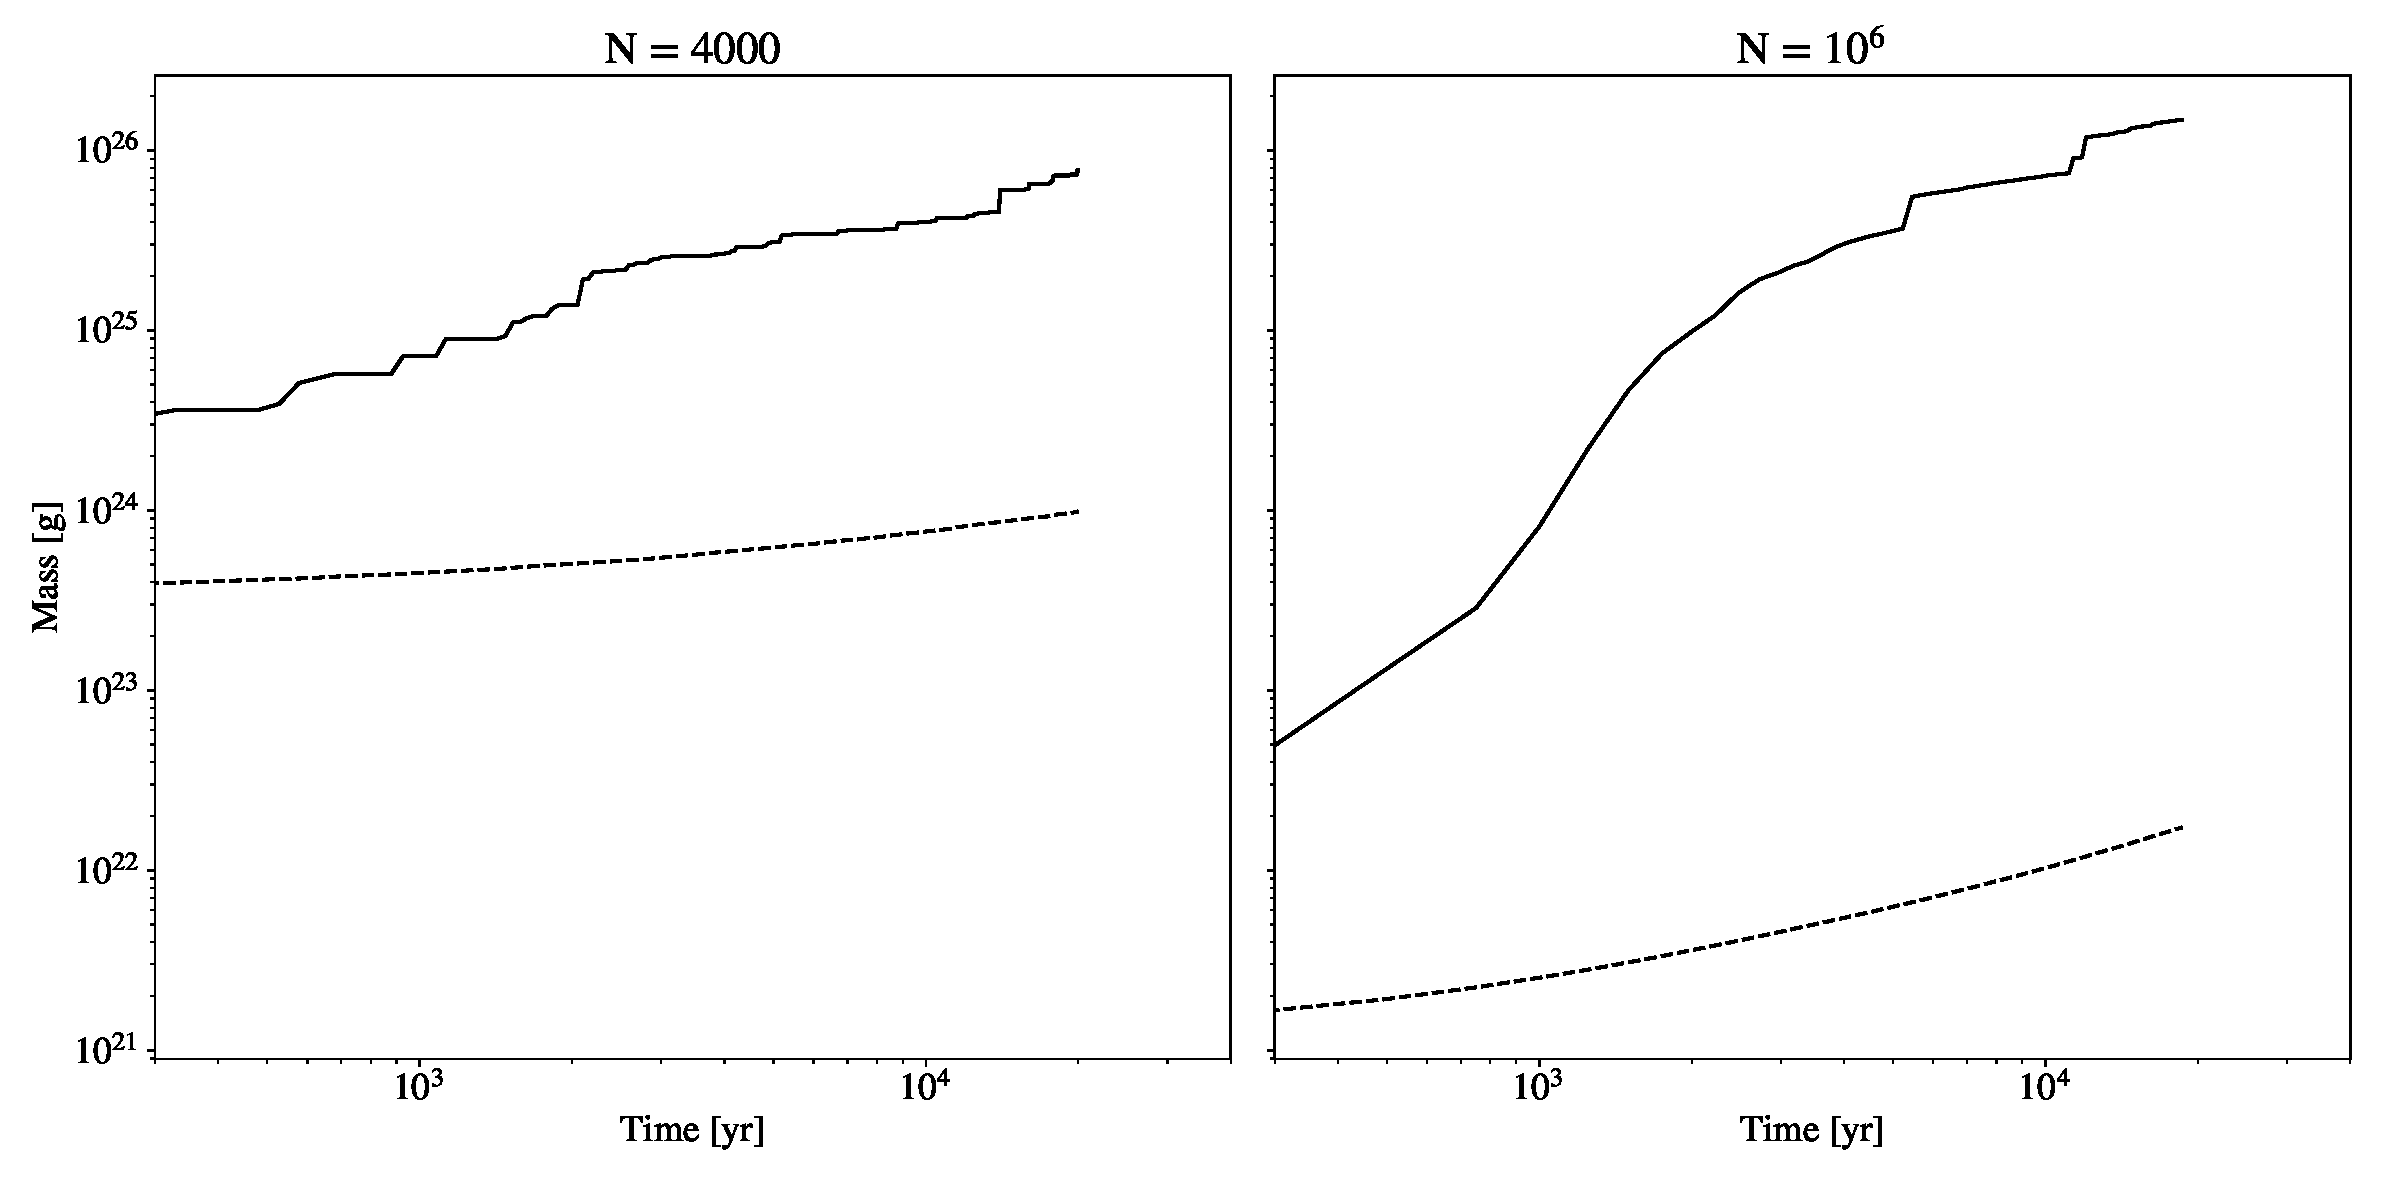
\includegraphics[width=\textwidth]{figures/plSS/mass_evo.eps}
    \caption{Evolution of the maximum (solid curve) and mean (dashed curve) planetesimal mass in the N=4000 and N=$10^6$ particle simulations. At early times, the maximum mass grows more quickly than the mean mass, which is indicative of runaway growth. After a few thousand years, the separation between the curves becomes a constant factor, signalling the start of oligarchic growth.
    \label{fig:mass_evo}}
\end{figure}

\begin{figure}
    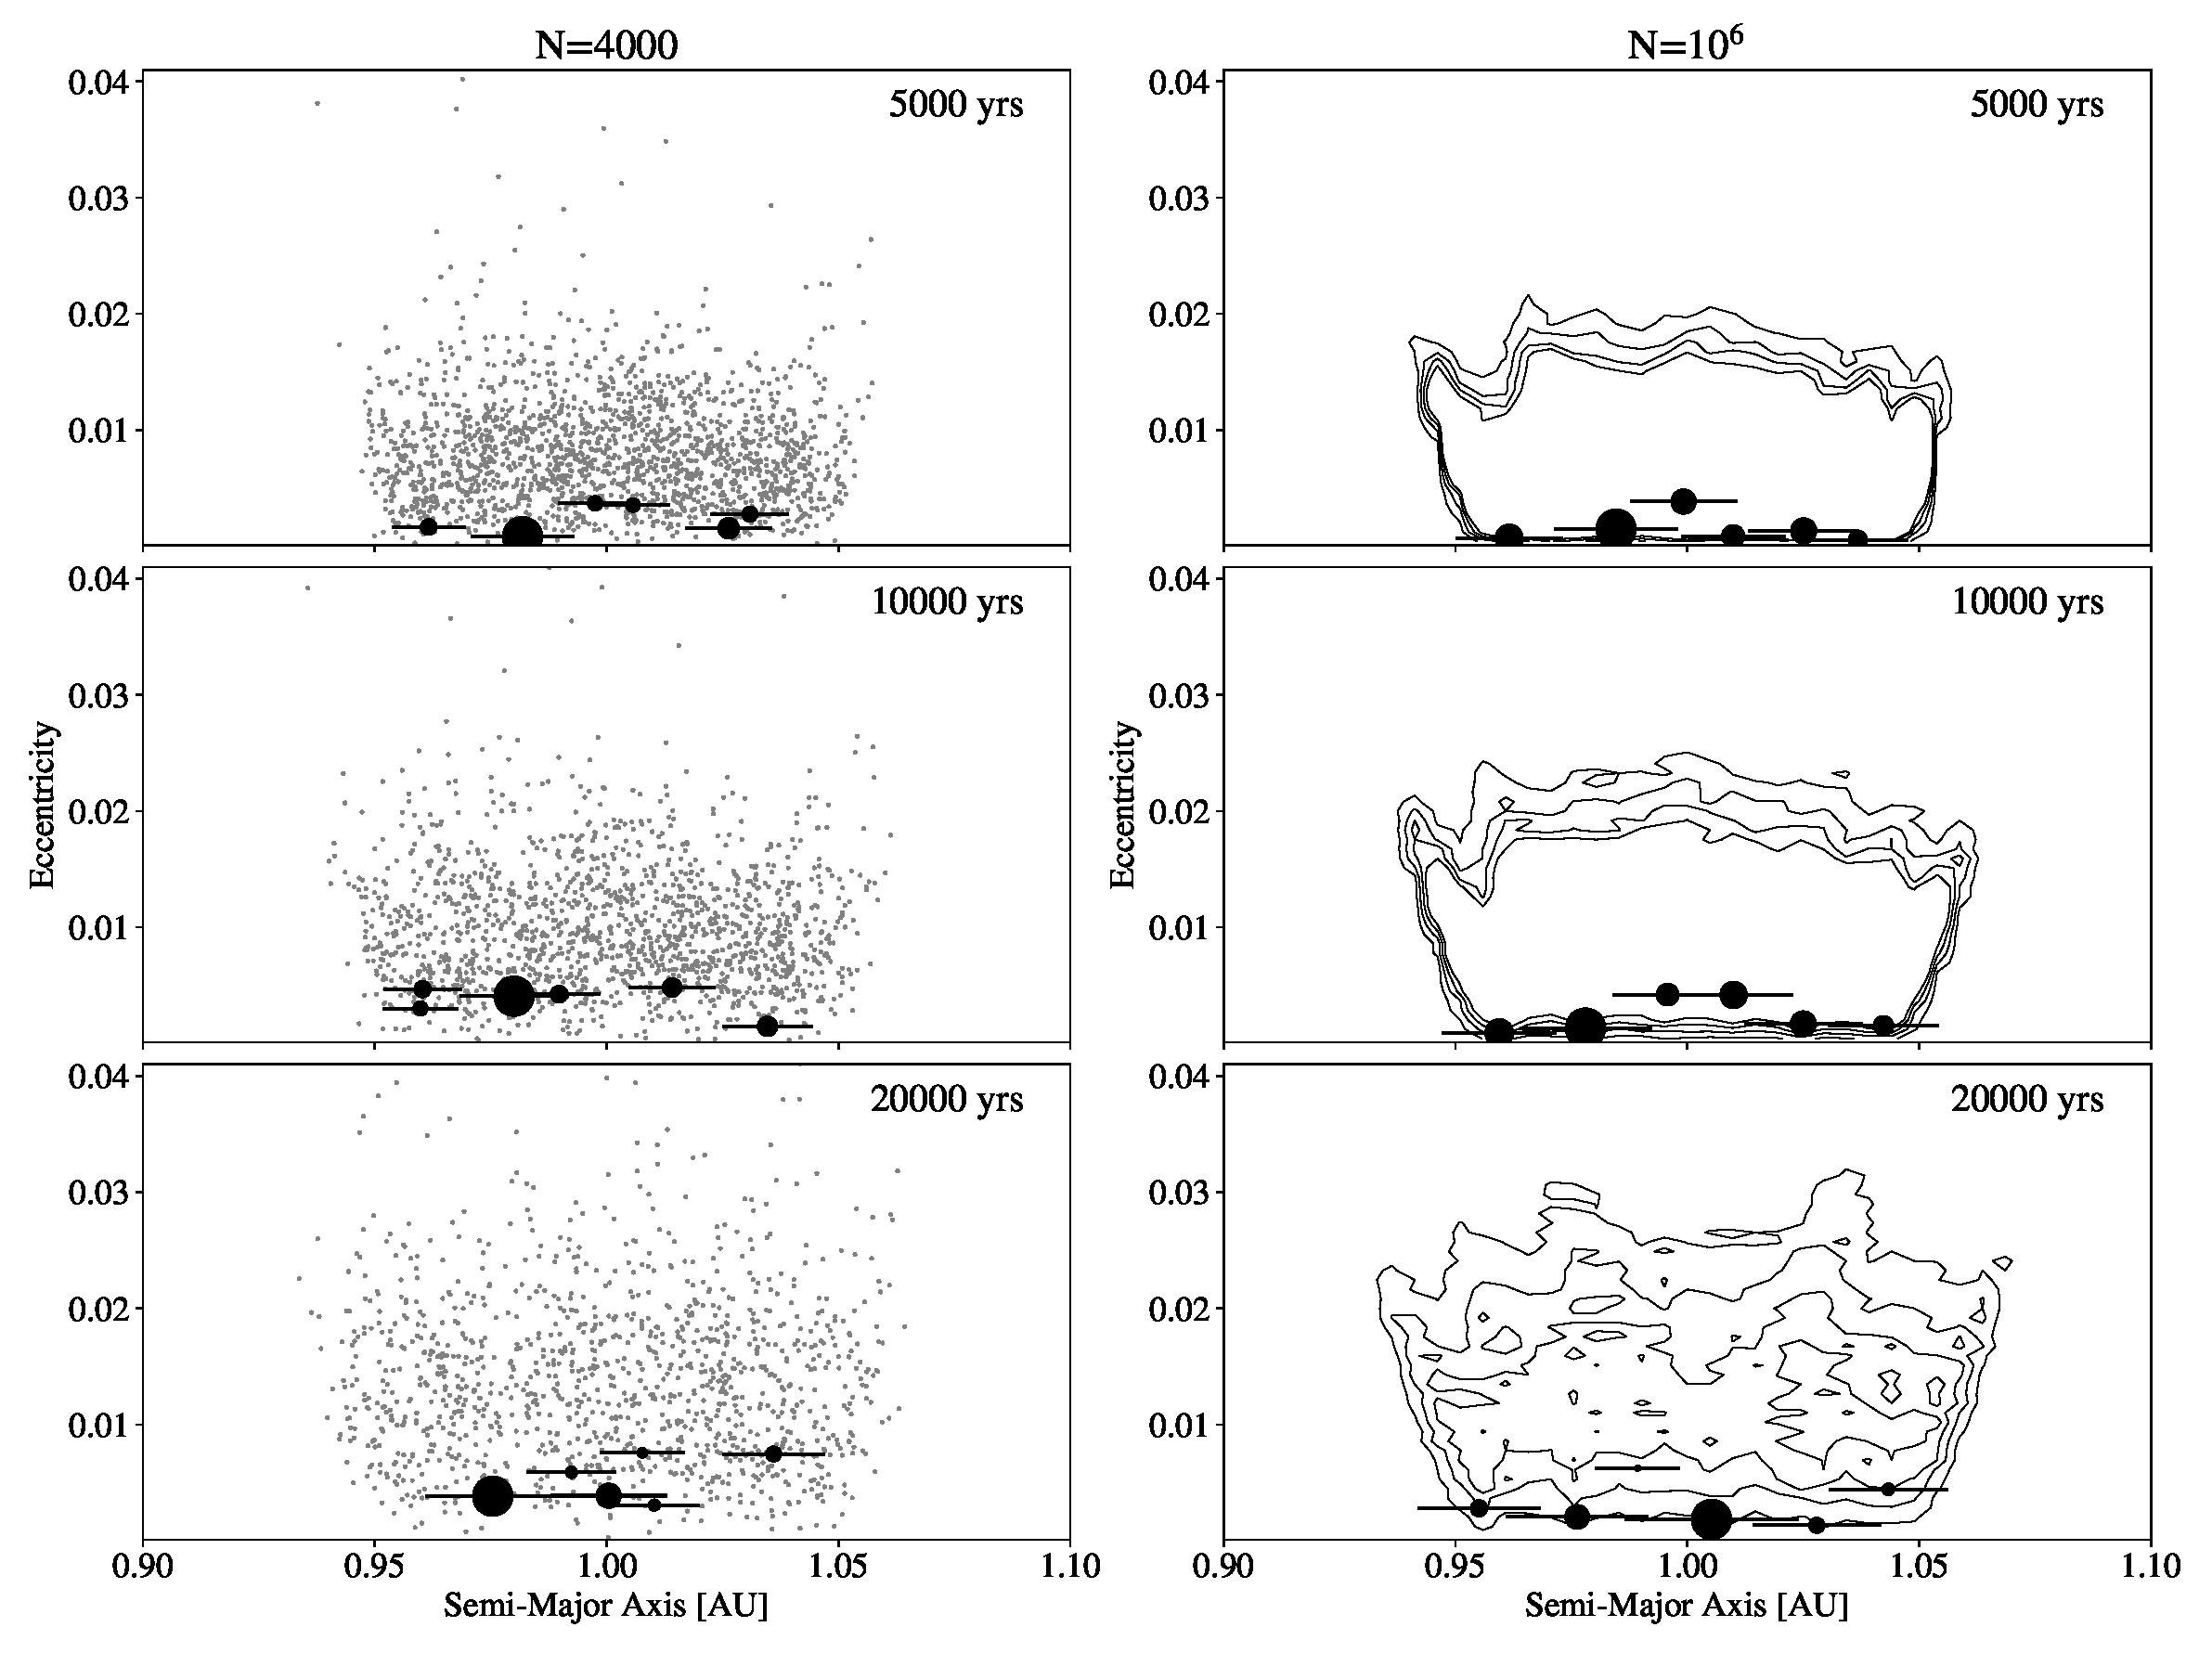
\includegraphics[width=\textwidth]{figures/plSS/ecc_evo.eps}
    \caption{Snapshots from the low and high resolution models in the $a-e$ plane. On the left, the light dots represent individual planetesimals, while the contours on the right hand plots represent curves of constant number density. The contour levels are the same between all panels and correspond to $7.8 \times 10^6$, $1.6 \times 10^7$, $2.3 \times 10^7$, and $3.1 \times 10^7$ planetesimals per AU per unit eccentricity. The black circles denote the configuration of the 6 largest bodies in the simulation, with the area of the circles scaled to the mass of the body. The horizontal error bars are scaled to 5 times the Hill radius of the bodies.
    \label{fig:ae}}
\end{figure}

\begin{figure}
    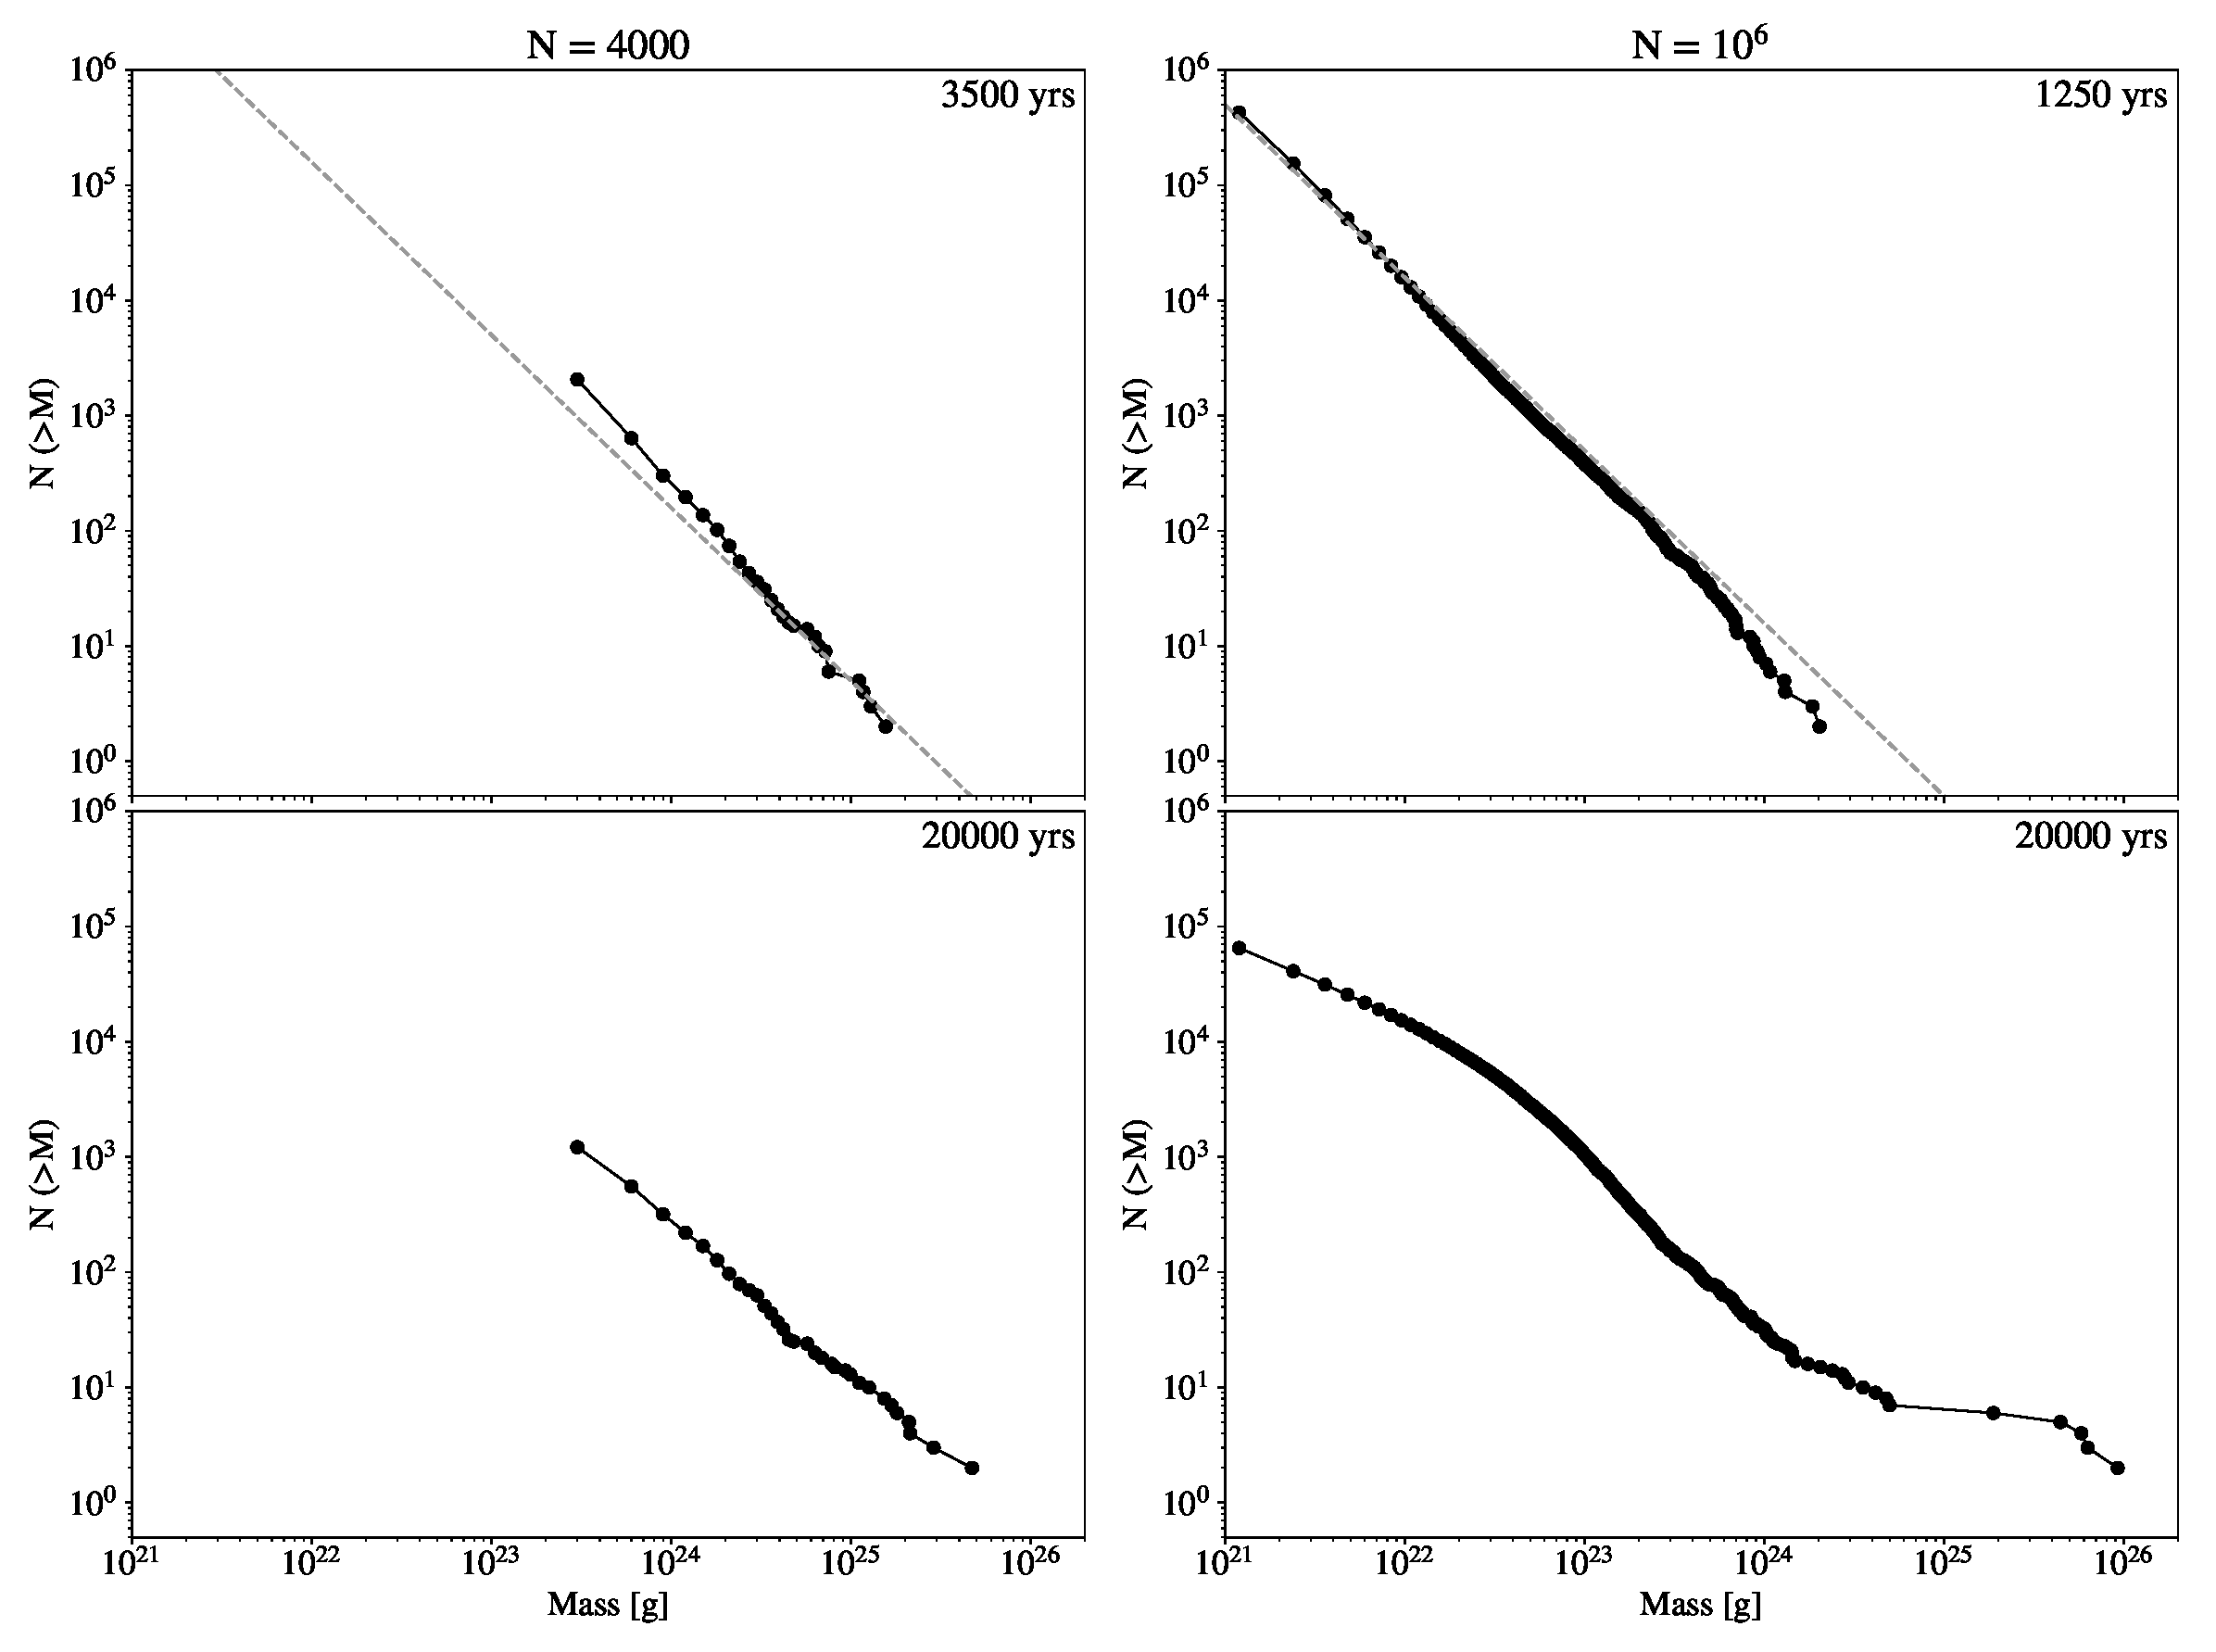
\includegraphics[width=\textwidth]{figures/plSS/mass_spectrum_evo.eps}
    \caption{Cumulative number of bodies in each mass bin for the low and high resolution runs, shown at the end of runaway growth (top row) and the end of the simulation (bottom row). The dashed line indicates a slope of -1.5, which is characteristic of runaway growth.
    \label{fig:mass_spectrum_evo}}
\end{figure}

\subsection{Initial Conditions} \label{sec:ics}

We begin by using our collision model to perform two sets of calculations:

(i) $10^{6}$ equal mass bodies with $m = 1.2 \times 10^{21}$ g

(ii) 4000 equal mass bodies with $m = 3 \times 10^{23}$ g

\section{Results} \label{sec:results}

\subsection{Low vs High Resolution}\label{sec:lowvshigh}

We begin by comparing the evolution of growth between the low resolution (N=4000) and high resolution (N=$10^{6}$) models. 
As planetesimals collide and grow, gravitational focusing becomes increasingly effective and the relative growth rate increases 
with mass \cite{greenberg78}. Figure \ref{fig:mass_evo} shows the evolution of the average and maximum planetesimal 
mass in both simulations. Runaway growth at early times is evident from the fact that the maximum mass grows more quickly 
than the mean mass. Eventually, the largest bodies begin to dynamically heat the neighboring planetesimals, which slows the 
growth rate of the largest bodies.

When gravitational focusing and dynamical friction are both effective, the growth rate of a planetesimal of mass $M$ is given by

\begin{equation}\label{eq:growth_rate}
\frac{dM}{dt} \propto \Sigma M^{4/3} e_{m}^{-2},
\end{equation}

\noindent where $\Sigma$ is the surface density of solid material and $e_m$ is the rms eccentricity of the planetesimals 
\cite{kokubo95}. Before the oligarchs form, the eccentricity dispersion is independent of mass and the fractional growth rate 
scales like $dM/dt \propto M^{4/3}$ \cite{wetherill93}. This implies that large bodies grow more quickly than small bodies, hence 
the runaway effect. Once the oligarchs form and dynamical friction becomes effective, energy equipartition causes the velocity 
dispersion to evolve toward $v_m \propto M^{-1/2}$\cite{ida93}. Using $v_m \propto e_m$ \cite{lissauer93}, the growth rate 
during the oligarchic growth phase scales like  $dM/dt \propto M^{2/3}$. Note that this does not imply that smaller bodies grow 
more quickly than large bodies. Rather, the growth rates tend towards the same value. This is reflected in figure 
\ref{fig:mass_evo}, where the slope of the maximum mass curve flattens out to match the slope of the mean mass curve after a 
few thousand years.

Comparing the two panels in figure \ref{fig:mass_evo}, it is also evident that the rate of growth is more vigorous in the high 
resolution case. This is due to the fact that the collision time-scale, given by 

\begin{equation}\label{eq:coll_timescale}
t_{coll} = \frac{1}{n \sigma v},
\end{equation}

\noindent is shorter in the latter case, where $n$ is the number density of planetesimals, $\sigma$ is the collision cross section 
and $v$ is the typical encounter velocity. The collision cross section depends on both the geometric cross section ($\propto 
N^{-2/3}$) and an extra term due to gravitational focusing ($\propto N^{-7/3}$), where $N$ is the total number of particles in the 
simulation and the total disk mass is fixed. Because the eccentricity and inclination dispersion (and therefore the scale height of 
the disk) are kept fixed between the low and high resolution simulations, the typical encounter velocity does not vary with $N$. 
Here, we retain only the leading order term for the collision cross section, in which case these quantities scale like $n \propto N$, 
$\sigma \propto N^{-2/3}$ and $v \propto const$ so that

\begin{equation}\label{eq:coll_timescale_N}
t_{coll} \propto N^{-1/3}.
\end{equation}

Figure \ref{fig:ae} shows the a-e distribution of planetesimals at three snapshots from both simulations. In both cases, the 
eccentricity dispersion grows as energy from Keplerian shear is transformed into random motion, an effect known as viscous 
stirring \cite{ohtsuki02}. The black circles denote the semi-major axis and eccentricity of the 6 largest bodies. The area of the 
circles indicates the mass of the bodies and the horizontal bars are each scaled to 5 times the Hill radius of the bodies. 
Gravitational scattering between the oligarchs, coupled with dynamical friction from the surrounding planetesimals, places the 
oligarchs on low eccentricity orbits that are spaced apart by a 5-10 Hill radii via orbital repulsion \cite{kokubo98}.

Next, we examine the evolution of the mass distribution of planetesimals. This is shown in figure \ref{fig:mass_spectrum_evo}. At 
early times, both models exhibit a power law distribution $N(<M) \propto m^{-p}$, where $p$ = 1.5 for the small bodies. A mass 
distribution with this slope is characteristic of runaway growth \cite{wetherill93}. The top panels show the mass distribution from 
both simulations at the end of the the runaway growth phase. In all subsequent snapshots, the mass distribution deviates from a 
single power law as the most massive bodies break away from the distribution, signaling the start of oligarchic growth. This 
happens sooner in the high resolution case. The bottom panels show the mass distribution at the end of the simulation at T = 
20,000 years.

Besides the fact that growth is more vigorous at higher resolution, the final mass distribution of planetesimals in the $N = 10^{6}$ 
case develops a feature that does not appear in the low resolution model. In the low resolution case, the low mass end of the 
mass distribution of planetesimals retains a single power law slope. The high resolution model, on the other hand, develops a 
bump in the mass distribution near $10^{22}$ g.

\begin{figure}
    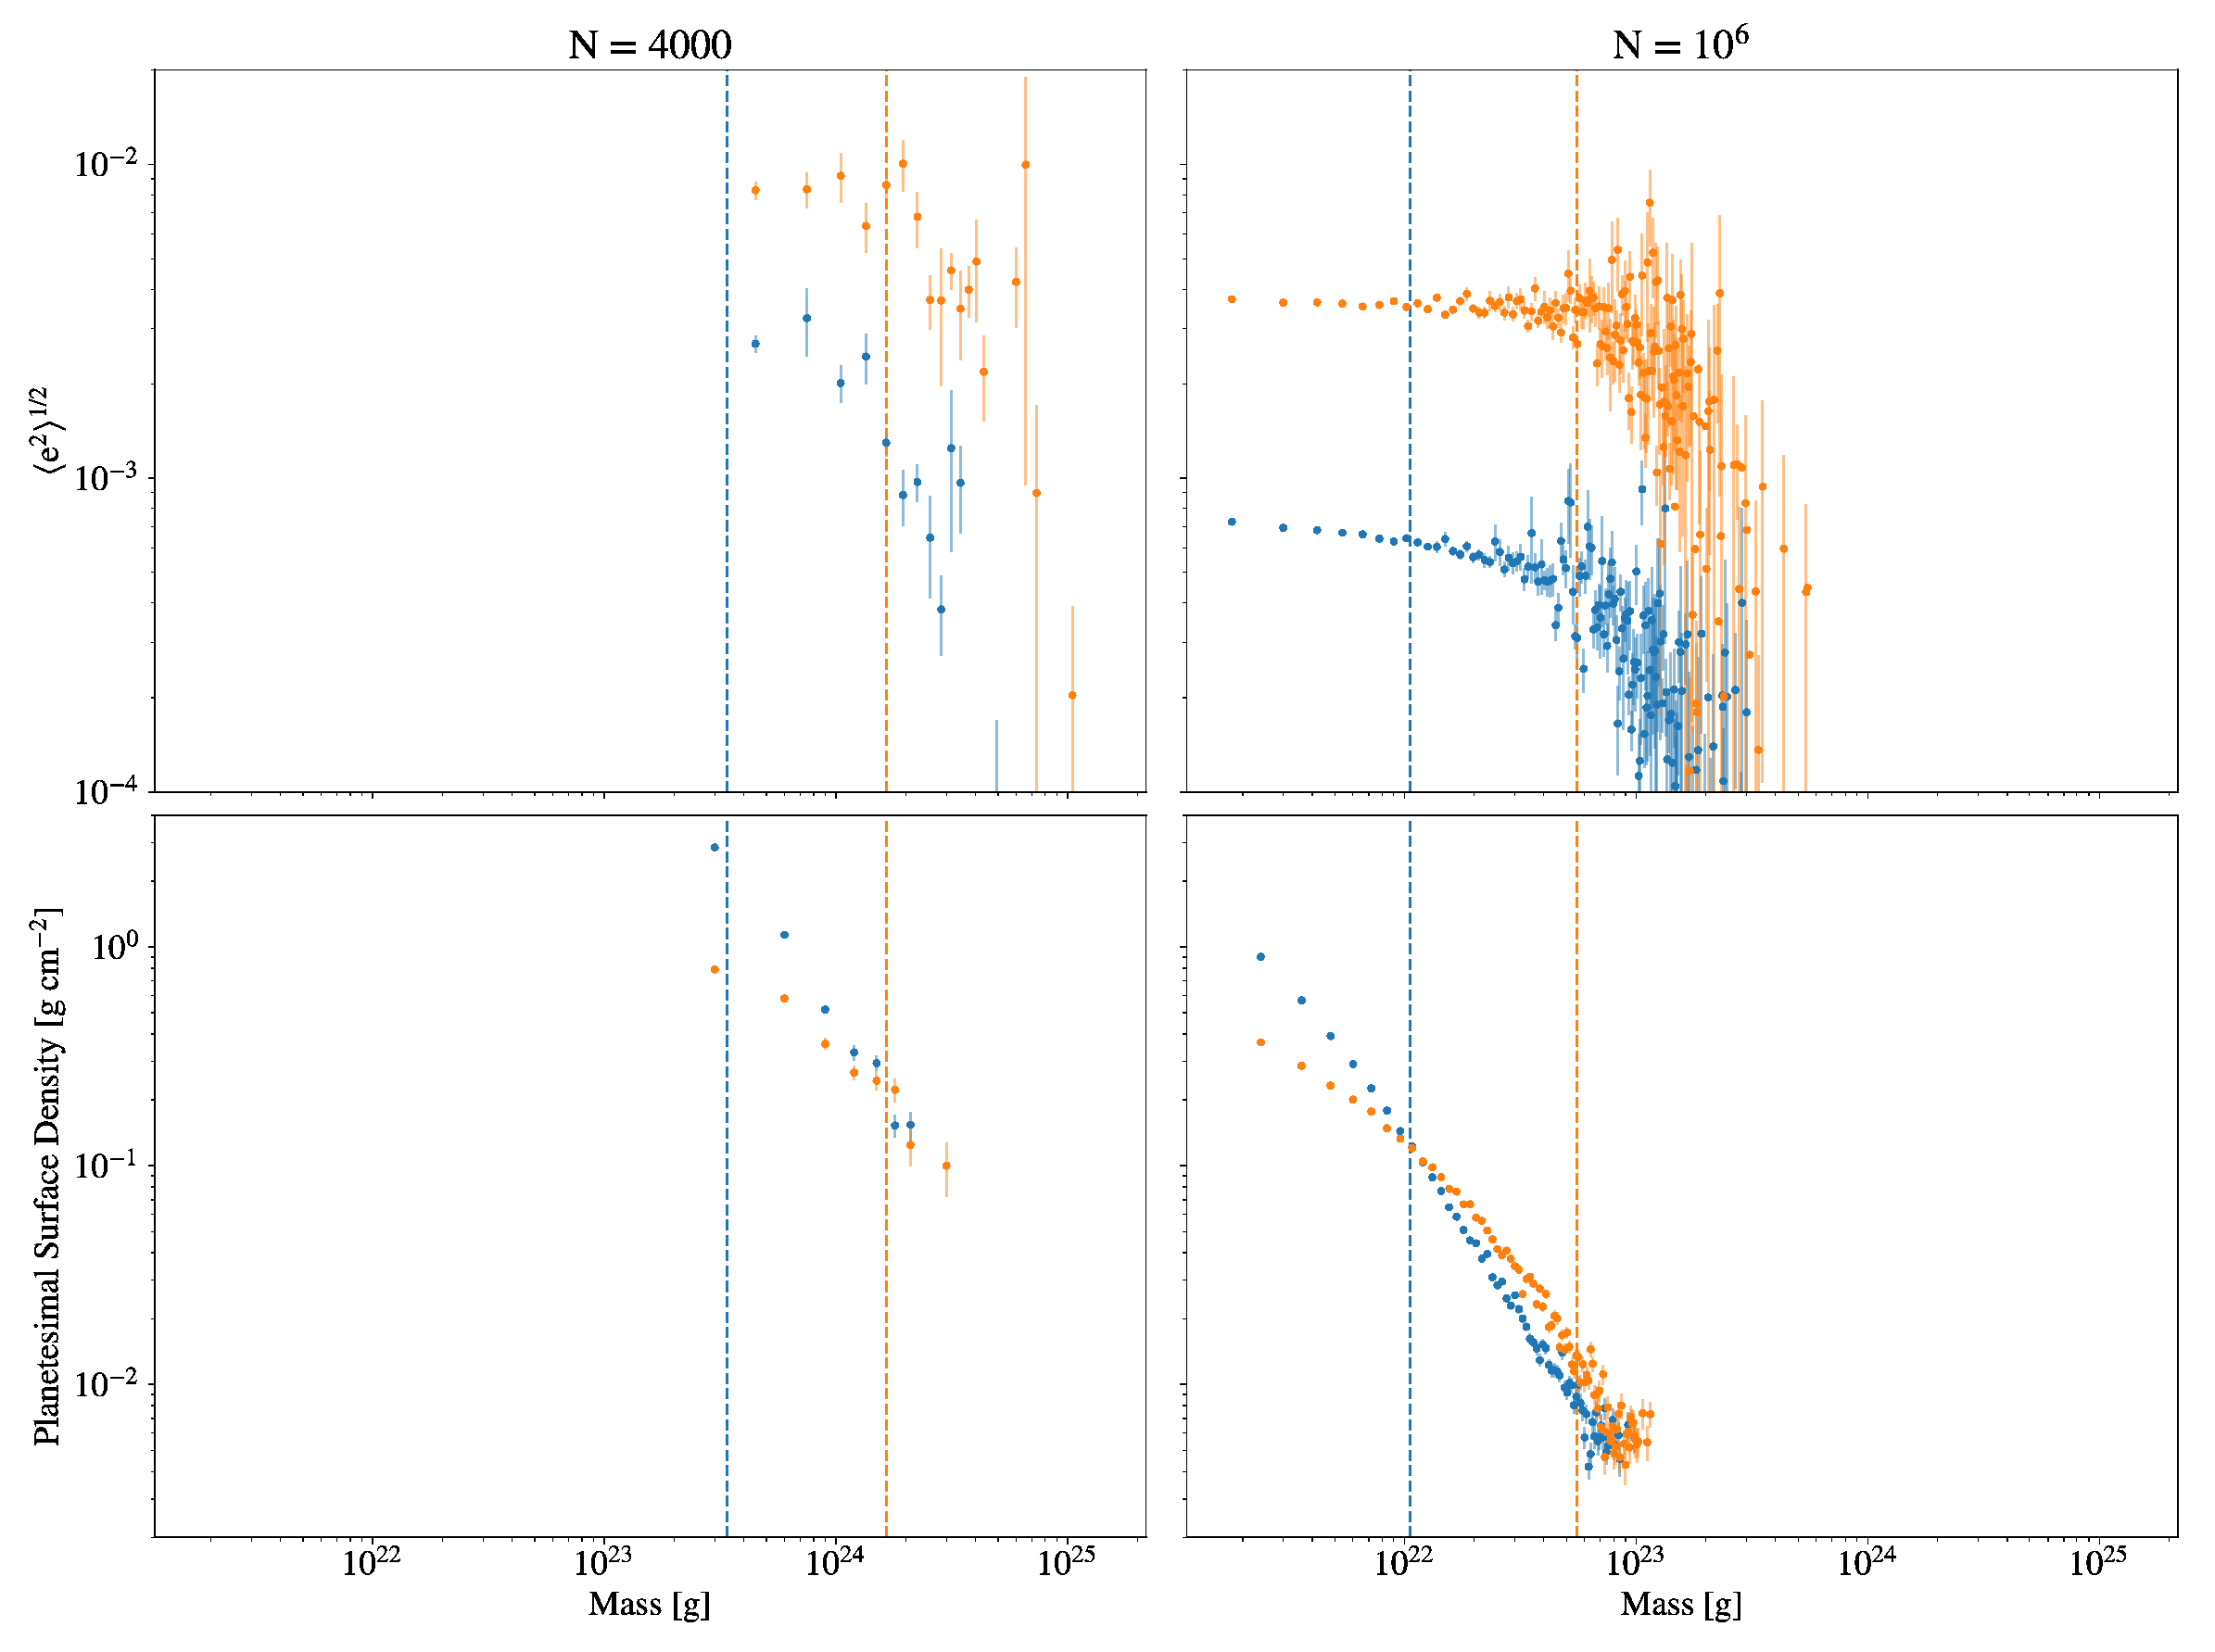
\includegraphics[width=\textwidth]{figures/plSS/ecc_den_evo.eps}
    \caption{The rms eccentricity (top) and planetesimal surface density at each mass (bottom) shown for the $N = 4000$ and 
    $N = 10^6$ simulations. The blue points correspond to the quantities at the end of the runaway growth phase (when the 
    mass distribution deviates from a single power law) and the orange points are from the end of the simulations (T = 20,000 
    years). The vertical dashed lines indicate the value of $M_{stir}$ during that snapshot.}
    \label{fig:ecc_den_evo}
\end{figure}

\subsection{Explaining the Bump in the High Resolution Mass Spectrum}\label{sec:bump}

We would next like to determine what produces the feature at $10^{22}$ g in the high resolution simulation and why it is absent 
from the low resolution run. Upon close inspection of the simulation snapshots, both models retain a mass distribution that 
follows a single power law up until the onset of oligarchic growth. The bump in the high resolution mass spectrum becomes 
visible shortly after the oligarchs form. Over the course of the simulation, the bump gradually becomes more prominent. Because 
the bump appears shortly after the first oligarchs do, its presence is likely tied to the formation of the oligarchs.

Other investigations of planetesimal growth have revealed a similar bump in the size frequency distribution (SFD) at intermediate 
masses. \cite{morbidelli09} found that the location of this bump was set by the initial size of the planetesimals. Objects smaller 
than this size were created through disruptive collisions, which resulted in a shallower slope on the SFD to the left of the bump. 
Our collision model does not allow for fragmentation, so we must look for another explanation.

\cite{wetherill11} showed that a bump in the SFD was an artefact of the transition between shear and dispersion dominated 
growth. Objects in the shear regime, whose encounter velocities are dominated by the differential rotation of the disc, grow more 
slowly than those in the dispersion regime, whose encounters are set by the random velocity dispersion. Because the velocity 
dispersion varies with planetesimal mass, both of these growth modes can operate simultaneously. Energy equipartition should 
cause the velocity dispersion to decrease with mass, so the transition between shear and dispersion dominated growth should 
happen at some intermediate mass. Finally, the smallest bodies have a velocity dispersion that exceeds their escape velocities, 
which sets a third, slow mode of growth in which gravitational focusing is ineffective. Although our high resolution simulation 
resolves all three modes of growth, we find that the boundaries between these modes smoothly and steadily evolve. Over the 
course of the simulation, the shear-dispersion boundary increases from about $10^{22}$ g to $10^{25}$ g, while the dispersion-
escape boundary evolves from about $10^{21}$ to $10^{24}$ g. Any artefacts that these boundaries would leave on the 
planetesimal mass distribution should get washed out, so we also rule these out as explanations for the $10^{22}$ g bump.

Although the boundary between shear and dispersion dominated growth does not seem to be producing the bump, there still 
must be some kind of transition between growth modes occurring near this mass. As shown by equation \ref{eq:growth_rate}, 
the growth rate is controlled by both the surface density of the planetesimals and their eccentricities. In figure 
\ref{fig:ecc_den_evo}, we show the rms eccentricity and surface mass density of the planetesimals as a function of mass at the 
end of the runaway growth phase (blue points) and at the end of the simulation (orange points). In this figure, each point 
corresponds to the relevant quantity calculated for all planetesimals with the exact same mass. Because the simulations start 
with equal mass planetesimals which grow via pairwise collisions, the masses take on discrete, linearly spaced values. We found 
that logarithmically binning the mass values alters the shape of the distributions, especially in the high resolution case where the 
quantities span many orders of magnitude. For this reason, we chose not to bin any of the data. The error bars in figure 
\ref{fig:ecc_den_evo} are obtained via 10,000 iterations of bootstrap resampling. For the high resolution simulation, the error 
bars at low mass are smaller than the size of the points.

The surface density was determined by calculating an azimuthally averaged density profile using the analysis package
{\sc PYNBODY} \cite{pontzen13}. The surface density for each planetesimal mass was taken to be the average surface density 
for those particles in a single radial bin from 0.9575 to 1.0425 AU, which spans the initial boundaries of the annulus.

One might expect that the rms eccentricity spectrum should eventually reach energy equipartition ($e \propto m^{-1/2}$), but this 
has been shown to only occur with a sufficiently steep mass distribution \cite{rafikov03}. In our case, the mass distribution is 
shallow enough that the velocity evolution of the low mass bodies is set only by interactions with large planetesimals. The mass 
below which this occurs, shown by the vertical dashed lines in figure \ref{fig:ecc_den_evo} is given by
\cite{wetherill93, ormel10}

\begin{equation}\label{eq:mstir}
M_{stir} = \frac{\left< m^2 \right>}{\left< m \right>}.
\end{equation}

Below this mass, planetesimals do not produce a dynamical friction wake and their velocity evolution becomes independent of 
mass \cite{rafikov03}. Because we started with equal mass planetesimals, the mass distribution was steep at early times. A 
power law slope steeper than $p = -2$ should produce a mass-dependent velocity distribution everywhere \cite{rafikov03}. In 
the top right panel of figure \ref{fig:ecc_den_evo}, the rms eccentricity distribution is not entirely flat below $M_{stir}$, which is 
likely due to the evolving mass spectrum. The analysis of \cite{rafikov03}, however, assumes a static mass spectrum.

At late times, a power law break in the surface density distribution forms near $10^{22}$ g in the high resolution simulation. 
Because the surface density is tied to both the mass distribution and the spatial distribution of planetesimals, it is difficult to learn 
anything else about the dynamics that are altering the growth rate from this information alone. We will examine this further in 
section \ref{sec:dynint}.

Given the power law break in the surface density distribution below $10^{22}$ g, we infer that there must be a dynamical 
mechanism at work that alters the collision rates of the low mass bodies. By the time that the $10^{22}$ g bump begins to 
appear, the planetesimals are sufficiently hot enough to render gravitational focusing ineffective (equation \ref{eq:growth_rate} is 
also no longer applicable). In this case, any additional heating actually increases the collision rate. Because this effect appears 
around the time of the onset of oligarchic growth, it likely has something to do with dynamical friction between the oligarchs and 
the planetesimals. In the next section, we examine how dynamical friction might be more effective with small planetesimals.

\section{Dynamical Friction and Resolution} \label{sec:dynfric}

Although the Chandrasekhar formula \cite{chandraesekhar43} contains no dependence on particle mass, the 'granularity' of the 
surrounding medium has been shown to influence the action of dynamical friction \cite{brunini07}. This is because the individual 
kicks from gravitational encounters become less frequent and more powerful at coarse resolution, introducing extra stochasticity 
as the system evolves toward energy equipartition. \cite{obrien06} showed that a finely resolved planetesimal distribution during 
the oligarchic growth phase produced planetary embryos with low eccentricities. They did not, however, examine the mass 
spectrum to see if the oligarchs were preferentially heating the smallest planetesimals. In addition, their simulations only 
contained a few thousand particles, while our high resolution run contains in excess of 200,000 bodies at the onset of oligarchic 
growth. Comparing the largest embryos at the end of simulation (i) to their results, we find that the largest embryo in our high 
resolution run has an eccentricity that is a factor of 2 smaller than the embryos produced by \cite{obrien06}.

In addition to altering the cumulative effect of close gravitational encounters, there is evidence that energy and angular 
momentum exchange through resonances is more effective with fine granularity. For example, in collisionless simulations of 
galaxies, \cite{weinberg07a, weinberg07b} showed that a minimum number of particles was required to populate 
resonances and couple the rotation of a bar to the central halo cusp through Lindblad resonances. If the resolution was too 
coarse, gravitational potential fluctuations would scatter particles out of resonances and prevent any strong torque between the 
bar and the halo. Likewise, \cite{cionco02} showed that resonant torque has a measurable effect on the interaction between a 
planet and a planetesimal disc.

\begin{figure}
    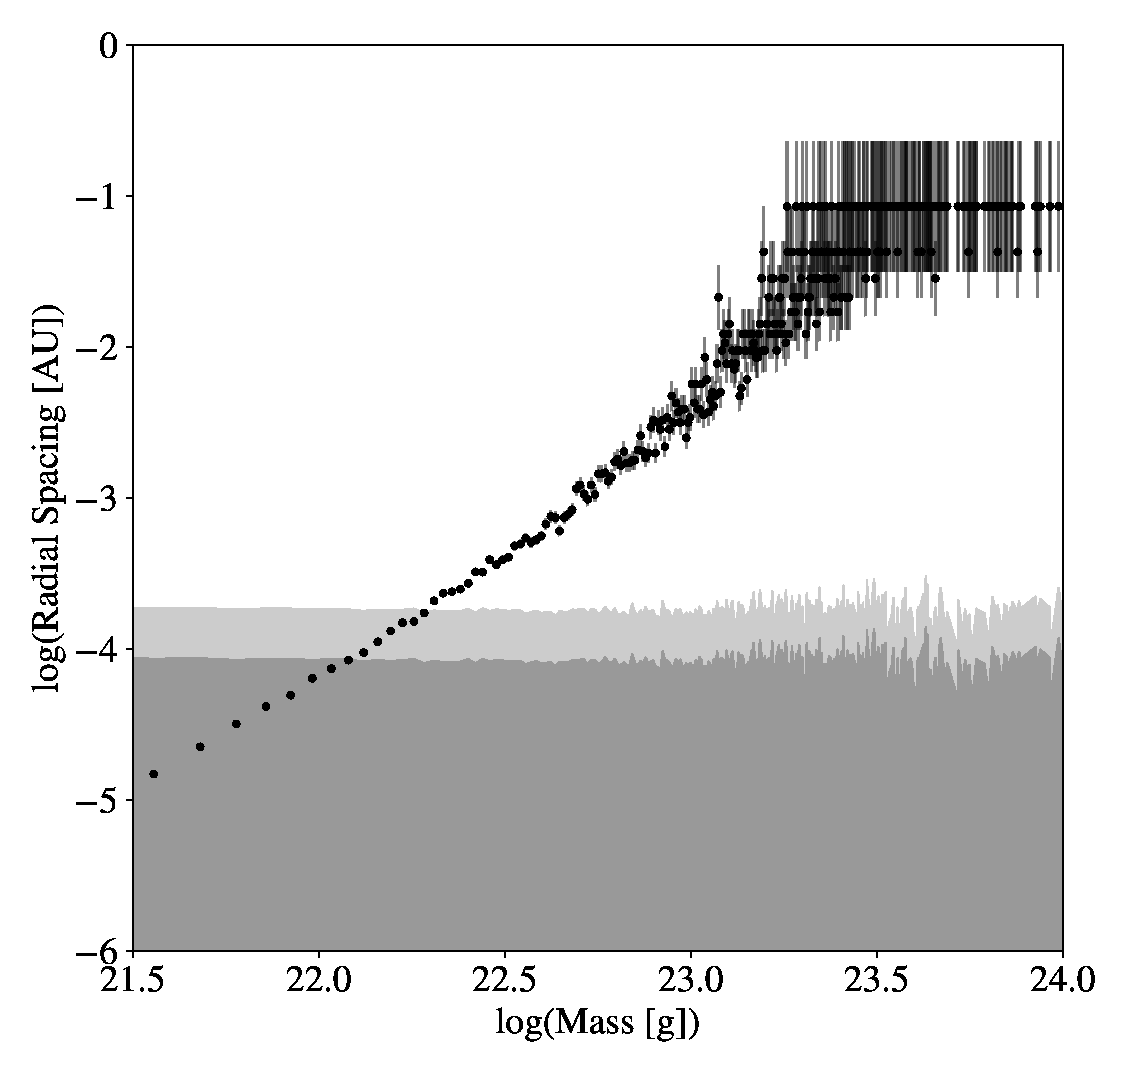
\includegraphics[width=\columnwidth]{figures/plSS/res_width.eps}
    \caption{The average spacing in semi-major axis as a function of mass at the end of the high resolution growth simulation 
    (black points). The gray regions indicate the libration width of planetesimals in each mass bin that are in resonance with the 
    most massive oligarch. The light gray region corresponds to the libration width of the 65:64 (highest non-overlapping) 
    resonance and the dark gray region corresponds to the 15:14 (most distant populated) resonance.}
    \label{fig:res_mass}
\end{figure}

\subsection{Resolved Resonances}\label{sec:resonances}

During the oligarchic growth phase, a handful of massive bodies lose energy and angular momentum to the surrounding 
medium. The previous runaway growth phase leaves behind a steadily varying spectrum of planetesimal masses, whose number 
decreases with mass. Assuming the planetesimals are randomly distributed throughout the disc, the granularity can be thought 
of as increasing with mass. This implies that the dynamical friction should be more effective from the smallest planetesimals. 
Because the planetesimals appear to be more strongly heated below a certain mass threshold, we hypothesize that the change 
in growth modes has to do with the activation of resonances, rather than a smooth decrease in the stochasticity of scattering 
events.

Because spiral features like those seen in \cite{weinberg07a, weinberg07b} and \cite{cionco02} are unlikely to form in such a 
narrow annulus, we will consider the effects of mean motion resonances (MMRs), which are a subset of the Lindblad resonances 
considered in the aforementioned studies. In order to determine the resolution required to resolve MMRs, we calculate the 
libration width of first order MMRs associated with the oligarchs and compare it to the average radial spacing between 
planetesimals as a function mass. The average radial spacing is given by

\begin{equation}\label{eq:spacing}
\left< \Delta r \right> = \frac{\Delta a}{N(m)},
\end{equation}

\noindent where $\Delta a$ is the width of the annulus and $N(m)$ is the number of planetesimals of each mass.